\definecolor{gainsboro}{rgb}{0.90, 0.90, 0.90}

\addchapheadtotoc
\chapter{Fundamentals}
The following chapter introduces basic terms and concepts that play an essential part in understanding the complexity of software security testing. It presents conventional approaches and briefly explains the approach taken in this thesis.

\section{Testing Approaches}
\subsection{Model Based Testing}
In the software development process, model-based testing describes the automated generation of test cases based on a formal model of the system under test (SUT). It checks the correctness of a system by performing experiments in a systematic and controlled way. \citep{torxAMBT2003}

Model-based testing is led by an oracle that runs assertions for test generation and execution.
The test oracle collects the results from the tests and creates reports out of it. \citep{sypolt2018}

\newpage 

\begin{figure}[ht!]
\begin{center}
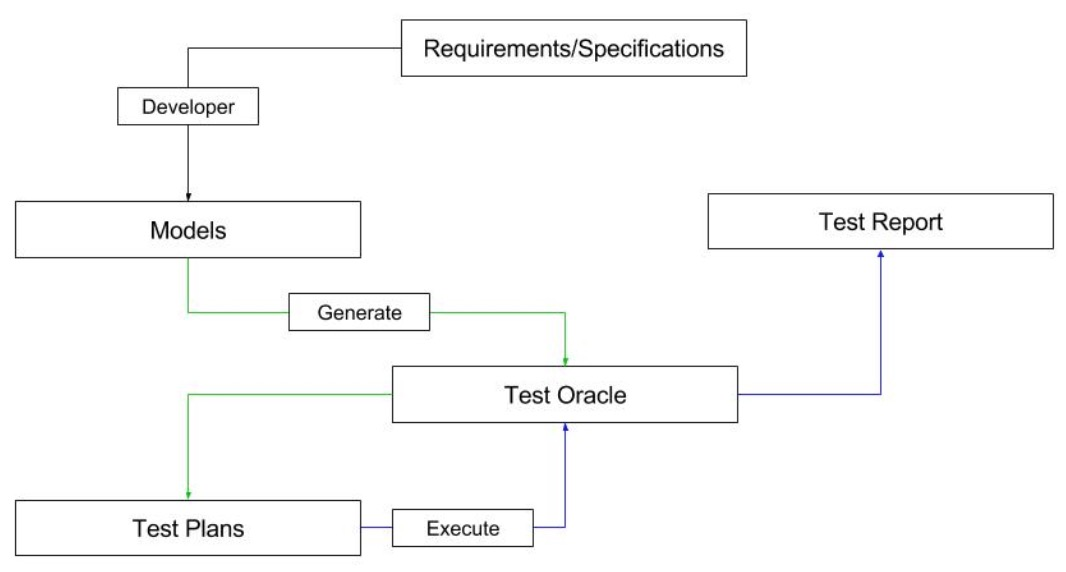
\includegraphics[height=8cm]{modelbasedtesting_sypolt.jpg}
\end{center}
\caption[Model Based Testing Schema - Role of the testing oracle]{Model Based Testing Schema - Role of the testing oracle. Graph from \citep{sypolt2018}}
%Source:
\label{fig_devsecops}
\end{figure}

The general rule with model-based testing is that the success of a given model is based on the quality of the model. \citep{mbsvt2007}
Functional models typically describe the behavior, while architectural models define the configuration of a system. \citep{mbst2012}
An example of the later will be covered in \ref{infrastructure_testing} using Azure Policies.

Model-based security testing (MBST), in addition to functional testing, consists of approaches such as model-based fuzzing, risk and threat oriented testing, and the usage of security patterns. MBST has a more complex scope since functional hazards, such as accidental mistakes on implementation, are simpler to find than persistent security threats. \citep{mbst2012}

Model-based vulnerability testing (MBVT) is an even more specific field of application for the model-based paradigm. \citep{mbsvt2007}
Vulnerabilities are mostly not related to the functional requirements of the application. Rather they are sensitive to implementation details, which requires thought-through planning. \citep{mbvtWA2013}


\subsection{Planning Based Testing}
\label{planningBased}
Testing based on planning is comparable to the model-based testing approach. The automatic generation of test cases also needs some model of the to be tested system. 
One of the differences is that planners (planning based tools) also create an attack plan and then transform the plan into suitable test cases \citep{wotawa2014}.

The concept of planners is common for intelligent agents and autonomous systems. Transitions, and action sequences, are generated that transition the agent from the initial state into the given goal state.
The objective of planning based security testing is to ensure that applications reliably handle well-known attack patterns by modeling the attack as a sequence of known actions that are carried out in a specific order.

Instead of finding new vulnerabilities, handling known attacks is the focus of a planning-based approach.
In \citep{wotawa2014} the authors introduce an algorithm called PLAN4SEC which makes use of an ordinary planner that is provided with a problem and domain description based on the Damn Vulnerable Web App (DVWA).

Below is an example of a generated testing plan of a given domain and problem description from \citep{wotawa2014}.

\begin{lstlisting}[ backgroundcolor = \color{gainsboro}, 
                    xleftmargin = 2cm, 
                    framexleftmargin = 1em, 
                    language=R,
                    caption={Planning Based Testing DSL Example},
                    captionpos=b]
0: START X URL LO
1: SENDREQ X LO SE SI
2: RECREQ X SI
3: PARSE X M USERNAME PASSWORD TYPE 
4: CHOOSERXSS X TYPE
5: ATTACKRXSS X XSSI M UN PW
6: PARSERESPXSS X SCRIPT RESP
7: PARSERESPXSSCHECK X SCRIPT RESP 
8: FINISH X
\end{lstlisting}

This generated plan is expressed in a domain specific language (DSL) which is parsed by JavaFF \citep{javaffColes}. The according Java functions for each instruction are then executed in order.

\subsection{Test Automation}
Even considering the existence of Model- and Planning based testing approaches, the most prominent approaches to testing are still manual \citep{secTestingSurvey2016}.
Replacing this repetitive manual execution by non-complex scripts and automation is the chosen approach in this paper.

Creating and establishing one of the more complex approaches requires specialized knowledge in both the domain and the abstraction process. The more common approach in software projects, see \ref{current_testing_etas}, is to either contract another department or company with the testing. Manually writing unit, integration, and regression tests for the most critical and feasible elements, as well as a Continuous Integration (CI) / Continuous Development (CD) pipeline for static code analysis, is also prominent \citep{secTestingSurvey2016}.

In the scope of vulnerability testing, for example, approaches like fuzzing, dir busting, and SQL injection can be used to find the so-called "low hanging fruit" and harden the project against very basic attacks \citep{autoPentestOverview2018}.

\newpage

\section{Security Testing}
\subsection{Compliance and Governance}
Compliance and Governance ensure the alignment of a given system with requirements, controls, and industry standards.
Even though they are both meant to protect an organization form the same threats and risks, they need to be looked at separately.

Both terms and concepts are crucial for understanding the role they play in the security testing process, as well as the importance of the Azure microservice implemented in this thesis.

\subsubsection{Compliance}
According to the Cambridge Dictionary, the term "compliance" describes the conformity of a system to a set of given rules and requirements \citep{compliance2020}.
This means that a system must meet those requirements in order to conform to the regulations and rules of the organization. 

In the context of software systems, requirements can be both organizational and technical. Organizational measures consider the conceptual requirements of a system, like defining and designing an access role concept. In contrast, technical measures define less abstract and more testable requirements like the state and format of logging in our applications. 

Compliance is only one of the conceptual entities combined in the process of Governance.

\subsubsection{Governance}
\citep{bannerman2009} describes Governance as "a multi-dimensional concept, encompassing elements of organizational stewardship, accountability, risk management, compliance, control, propriety, functional oversight, resource allocation, and capability. It tends to be defined from one of two perspectives: functionally, in terms of what Governance does (e.g., assigning and administering decision rights, responsibilities, and accountabilities) or; structurally, in terms of what it looks like (a framework of interrelated boards, councils, and committees)."

In the domain of software development, Governance can be described as a mechanism to ensure that defined engineering and business needs are met. Software development governance defines processes for "the assignment and maintenance of software development capability decision rights, governance responsibilities and accountabilities; software development capability planning, monitoring and review processes; issue escalation procedures, and stakeholder consultation" \citep{bannerman2009}.


\subsection{Static Application Security Testing (SAST)}
The "Static Source Code Analysis", as the name suggests, is performed without executing the program. It is a fundamental approach to review the formal correctness, data-flow, and even credential leaks.
Static code analysis is generally implemented as one of the first gates of continuous integration pipelines.

Depending on the focus of the analysis, there are different state-of-the-art providers for static code analysis like for example credential checking on Open-Source platforms like GitHub using GitGuardian \citep{gitGuardian2020}.

When focusing on security testing with static analysis, problems that can be identified with high confidence have to be targeted. Those include, for example, SQL Injections and Buffer Overflows.
The OWASP-project provides a list of tooling that can \citep{owaspStaticTools2020} be used as part of a continuous integration pipeline. 
Once a vulnerability is found, the build fails and provides detailed reporting to the developers who have to fix the issues before future builds succeed.

However, this approach has many drawbacks. It has a high rate of false positives, which can significantly increase the time needed for manual testing and reviewing.
In addition to that, most security vulnerabilities are difficult to find automatically. Access control issues or the insecure use of cryptography are only a few examples. Even misconfigurations cannot be identified without a model-based approach, as discussed before.

A more recent approach, Semmle QL, uses variant analysis to find problems in code based on a similar, known vulnerability. Code is treated as data and fed into the CodeQL engine together with custom queries that perform data analysis and track down known vulnerabilities \citep{semmle2020}. 

A straightforward query for finding all the comments that contain a \enquote{TODO} looks like the following.

\vskip 1cm

\begin{lstlisting}[ backgroundcolor = \color{gainsboro}, 
                    xleftmargin = 2cm, 
                    framexleftmargin = 1em, 
                    language=SQL,
                    caption={Semmle QL TODO Query},
                    captionpos=b]
import python

from Comment c
where c.getText().regexpMatch("(?si).*\\bTODO\\b.*")
select c
\end{lstlisting}


Much more complex queries for cases such as buffer overflows, critical recursion, or DOM XSS attack vectors are available. 
This approach enables more in-depth static analyses that can eliminate common known vulnerabilities.


\subsection{Functional security testing (FST)}
In the context of software development, functional testing can cover different scopes. When done in an isolated environment rather than an operational context, it is called "Unit Testing". When tested together with other applications of the system, it is called "Integration Testing" \citep{warren2011}.

Functional security testing, on the other hand, is focused on ensuring that applications do not act in ways they are not meant to, regardless of the scoping. The critical element of this approach is "Negative Testing," which tests explicitly for misbehavior, for example, on the corrupted or wrong input. Given the vast amount of attack vectors, this is a broad and open-ended task.

According to \citep{warren2011}, this approach can give some level of assurance in terms of the avoidance and resistance to attacks.


\subsection{Security Vulnerability testing (Penetration Testing)}
\label{securityVulnerabilityTesting}
According to \citep{mcgraw2006}, "Penetration Testing is a comprehensive method to test the complete, integrated, operational, and trusted computing base that consists of hardware, software, and people."

It is an analysis of the system for potential vulnerabilities such as hardware and software flaws and faulty system configuration. Even operational weaknesses and employee manipulation, with so-called Social Engineering, can be in scope for the test \citep{mohanty2020}.

Given the strong fan-out of attack vectors, penetration testing requires highly skilled candidates with a particular skillset focusing on the to be tested infrastructure and application \citep{bacuidoYuanChuJones2011}.

Penetration testing is different from functional security testing in a way that FST checks the correct behavior of the system's security controls. Penetration testing, in contrast, determines the difficulty for someone to penetrate an organization's security controls \citep{autoPentestOverview2018}.

In a study conducted by the German Federal Office for Information Security \citep{bsiStudy2020}, the five phases of the Penetration Testing process are defined as follows.

\begin{figure}[ht!]
\begin{center}
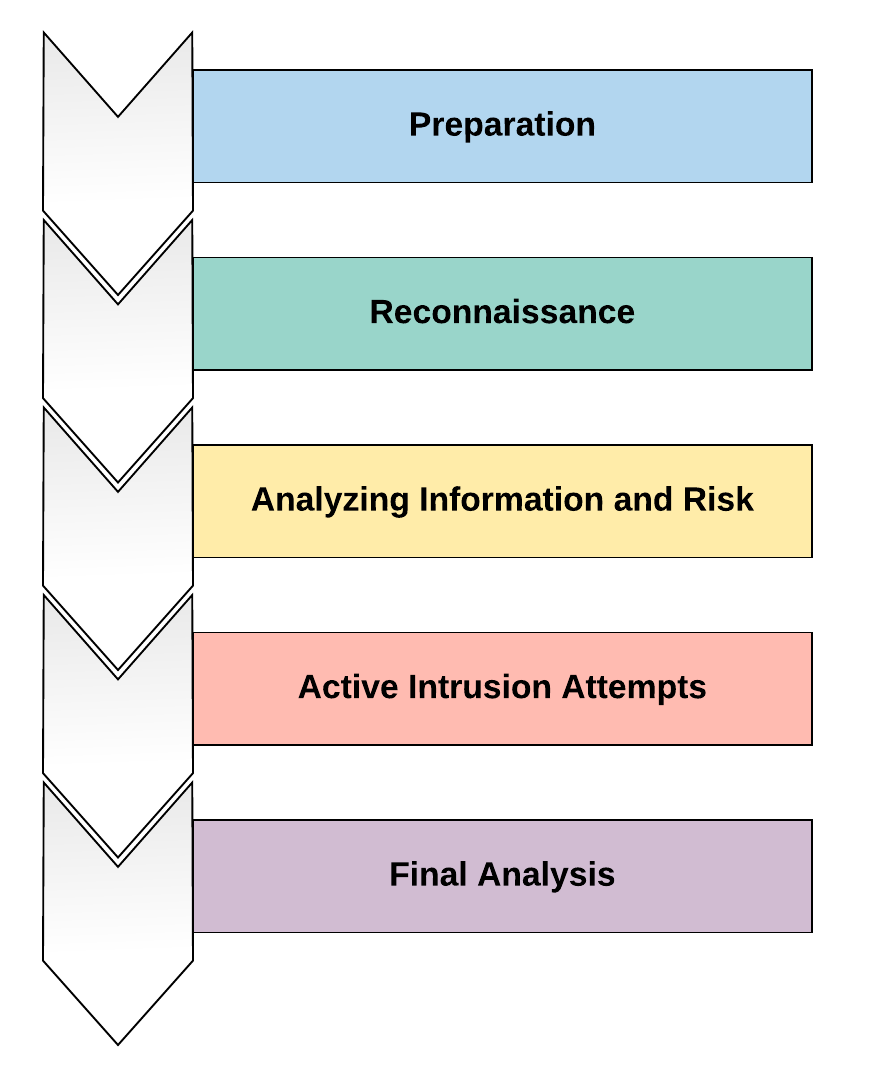
\includegraphics[height=10cm]{Pentesting_Process.png}
\end{center}
\caption[Penetration testing process flow - according to \citep{bsiStudy2020}]{Penetration testing process flow - according to \citep{bsiStudy2020}}
%Source:
\end{figure}

\newpage

\subsubsection{Phase 1: Preparation}
In the first phase, requirements and objectives, as well as procedures of the test, have to be defined with the client. The project has to be scoped and should be written down in the contract to avoid any legal infringements.

\subsubsection{Phase 2: Reconnaissance}
Reconnaissance is a strategic observation. In the second phase, a complete and detailed overview of the system, including possible attack vectors, is gathered and documented.

\subsubsection{Phase 3: Analyzing information and risks}
Phase 3 can act as a funnel to further filter down possible targets. The process of Threat and Risk Analysis (TaRA), as it is called at the security consulting team at the ETAS GmbH, includes defined goals for the test, potential risks to the system, and an estimate of the time required for system evaluation. 

\subsubsection{Phase 4: Active intrusion attempts}
Given the outline and analysis from previous phases, this phase covers the attack on the defined system to the in the analysis defined extend.

On systems with high availability or integrity requirements, potential adverse effects have to be considered in advance. For those systems, patches to prevent full system failures might be installed before testing. 

\subsubsection{Phase 5: Final analysis}
The last phase defines the requirements for report generation. The final report should "contain an evaluation of the vulnerabilities located in the form of potential risks and recommendations for eliminating the vulnerabilities and risks". It also has to disclose the done tests and found vulnerabilities. \citep{bsiStudy2020}


This manual process is time and resource-intensive while parts of it, especially reporting, are highly repetitive and display a high potential of automatability \citep{passi2018}.


\newpage

\section{Automated Testing}
\subsection{On the need for Automated Testing}
With the alarming amount of data breaches in recent years \citep{dataBreaches2019}, the need for security testing is more profound than ever before.
Many projects and even companies do not have access to security professionals due to the low number of available specialists and the time and cost intensity of such tests \citep{autoPentestOverview2018}.
Automated security testing, e.g., testing phases integrated into a continuous integration pipeline, could help to roll out underlying security testing mechanisms on a large scale.
Re-runnable and, especially, reproducible security testing as part of the release process that provides detailed automated reports can drastically increase the basic level of security of an application without the need for security specialists. \citep{vijayan2019}.

One of the biggest challenges for automated testing, however, is the absence of a strict model of the system. Without a formally given configuration of the system, deciding what is wrong or right relies on human decisions. There is no strict right or wrong in some cases \citep{mbst2012}.
Completely removing manual testing, as of now, is not feasible since automated processes do not have the intuition and lateral thinking of a human tester \citep{portswigger2020}.


\subsection{Automated Resource Compliance Testing with Policies}
\label{infrastructure_testing}
Since cloud resources, most of the time, are declared through a process called Infrastructure as Code, we have a specific model and reproducible configuration to base the testing on. 
These so-called templates define e.g., the type of the resource, the version, and properties like the amount of storage and CPU. Every attribute of the resource is defined through this configuration \citep{awsIac2017}. If values are not defined, they are assigned a set default value.

The structure and elements of such a configuration depending on the platform or cloud provider. For Microsoft Azure, the resource management system enables the use of e.g., built-in validation, policies as code, and CI/CD integration \citep{azureResourceTemp2020}.

A very simple example of such a resource manager template can look like this:

\begin{lstlisting}[ backgroundcolor = \color{gainsboro}, 
                    xleftmargin = 2cm, 
                    framexleftmargin = 1em, 
                    language=JSON,
                    caption={Microsoft Azure Resource Manager VM Template Snippet},
                    captionpos=b]
{
  "$schema": "https://schema.management.azure.com/schemas
              /2015-01-01/deploymentTemplate.json#",
  "contentVersion": "1.0.0.0",
  "resources": [
    {
            "type": "Microsoft.Compute/virtualMachines",
            "apiVersion": "2019-03-01",
            "name": "simpleLinuxVM",
            "location": "[resourceGroup().location]",
            "properties": {
                "hardwareProfile": {
                    "vmSize": "Standard_B2s"
                },
                ...
            }
        },
        ...
  ]
}
\end{lstlisting}

The above-displayed configuration is far from complete. However, it displays enough information to communicate the basic structure of such a template file. The templates create a new "B2s" computing instance and assign it to the location of the resource group. Properties like whether file encryption is active or if backups are enabled can, therefore, be checked using Azure Policies. Amazon Web Services has a comparable system called AWS CloudFormation templates \citep{awsCloudFormation2010}. The capabilities are similar, the format, however, is a little bit different.
A comparable configuration, like the one shown for Microsoft Azure, for AWS looks like this:

\begin{lstlisting}[ backgroundcolor = \color{gainsboro}, 
                    xleftmargin = 2cm, 
                    framexleftmargin = 1em, 
                    language=JSON,
                    caption={AWS EC2 Instance Template Snippet},
                    captionpos=b]
{
    "AWSTemplateFormatVersion": "2017-01-09",
    "Description": "Launch an EC2 Instance with 
                    defined properties",
    "Resources": {
        "SecureInstance": {
            "Type": "AWS::EC2::Instance",
            "Properties": {
                "ImageId": "ami-31814f58",
                "InstanceType": "t2.nano",
                "KeyName": "key-pair",
                ...
            }
        },
        ...
    }
}
\end{lstlisting}

With the given configuration, we launch a new t2.nano EC2 computing instance with the given properties set.

Using the Infrastructure as Code approach brings many more advantages than trivial compliance testability of resources. Reproducibility, management, monitoring, and optimization are streamlined through this code-centric approach \citep{awsIac2017}.

\begin{figure}[ht!]
\begin{center}
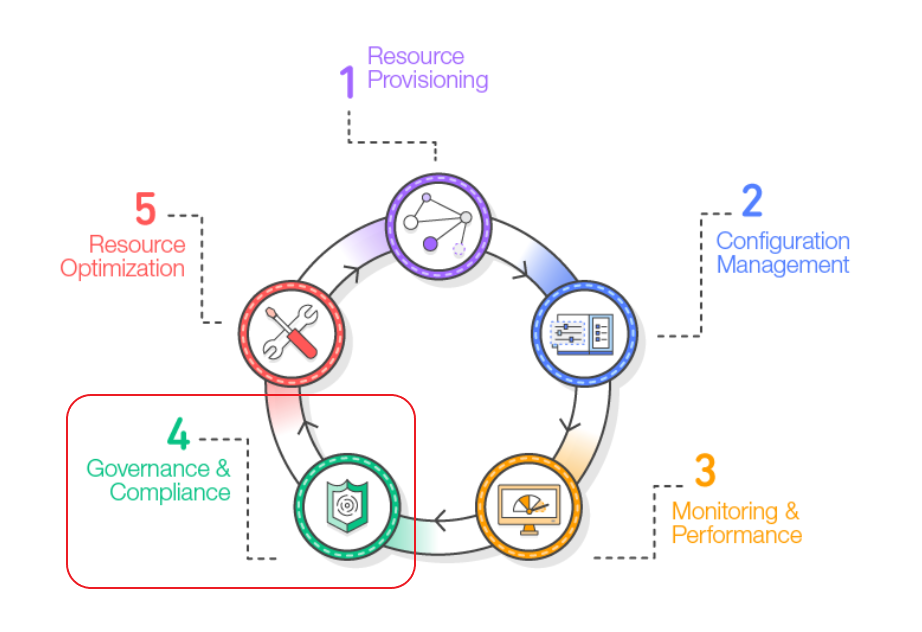
\includegraphics[height=8cm]{annotated_aws_iac_lifecycle.png}
\end{center}
\caption[Infrastructure resource lifecylce according to AWS]{Infrastructure resource lifecylce according to AWS. Drawing from \citep{awsIac2017}}
%Source: https://d0.awsstatic.com/whitepapers/DevOps/infrastructure-as-code.pdf
\label{fig_devsecops}
\end{figure}

Policy compliance testing for cloud resources is one of the processes for which a concept of automation was implemented in this thesis. Advance to \ref{automated_infrastructure_testing} to read about the concrete implementation further.

\newpage

\subsection{DevSecOps}
The concept behind DevSecOps integrates automated security testing into the continuous quality assurance of continuous development, integration, and deployment. 
It combines Development, Security, and Operations to improve the speed, turnover time, and overall quality of products.
Manual security and compliance testing slows down release processes and therefore needs to be augmented with automated testing and integrated into the continuous software deployment lifecycle.

\begin{figure}[ht!]
\begin{center}
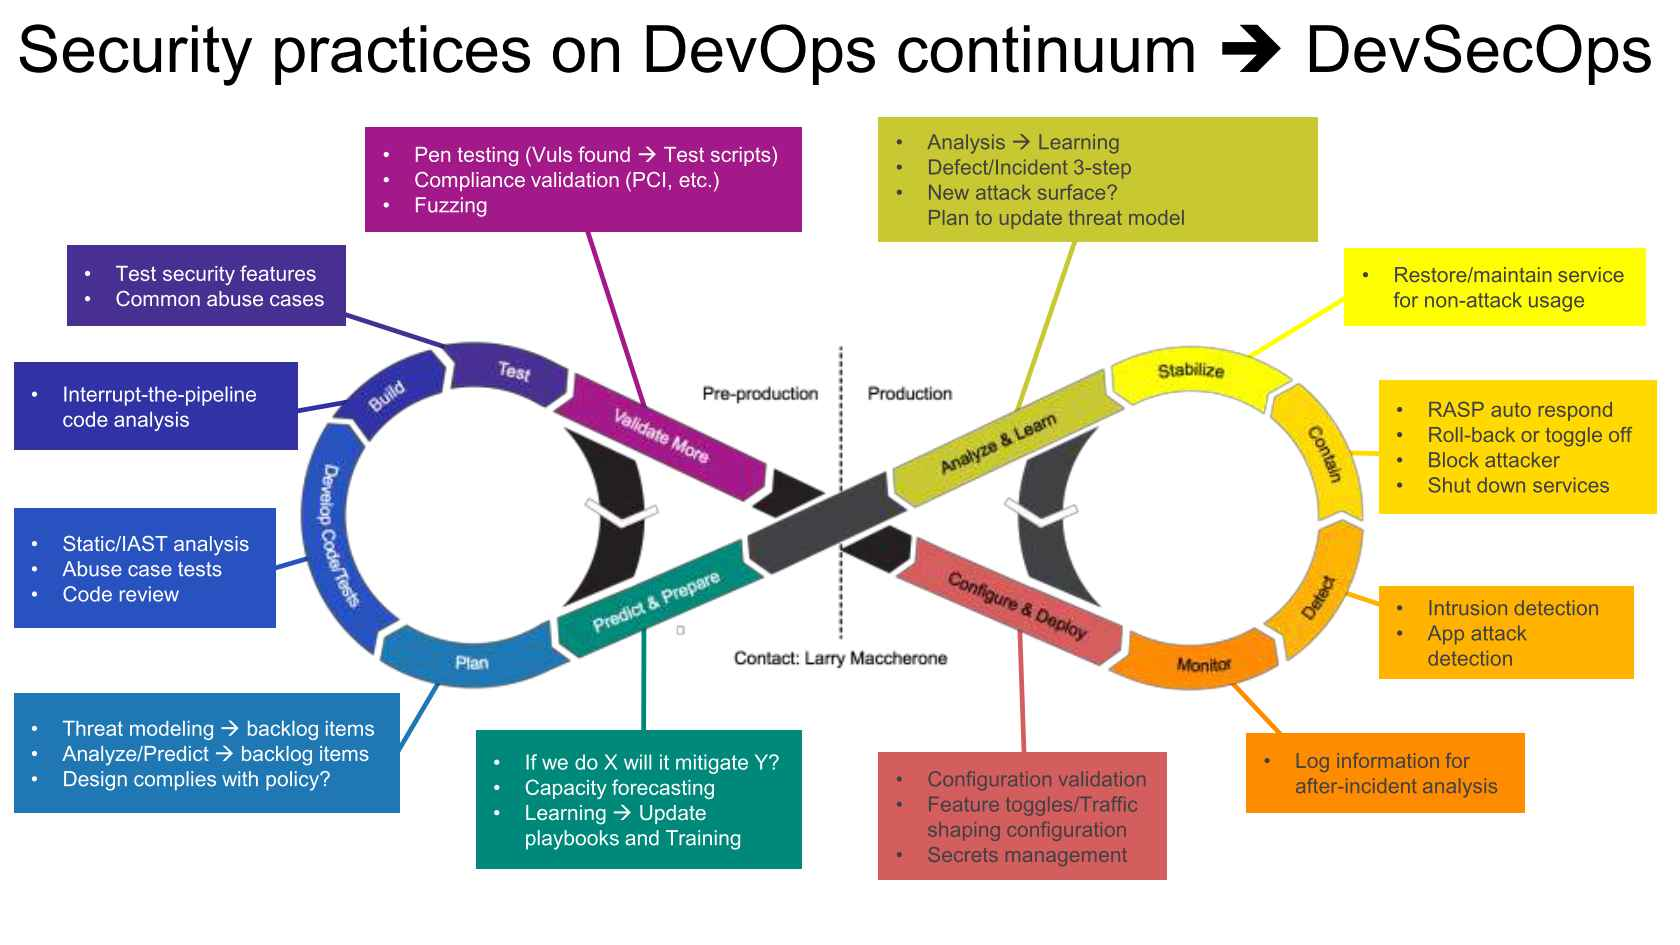
\includegraphics[height=8cm]{devsecops.jpg}
\end{center}
\caption[DevSecOps - Security practices on DevOps continuum]{DevSecOps - Security practices on DevOps continuum. Graph from \citep{alicloud2018}}
%Source:
\label{fig_devsecops}
\end{figure}

The schematic drawing of DevSecOps displays and explains the significant elements of the life cycle.
Security is implemented in the overall process, and breaches in security or compliance lead to interrupted releases.
In the operations phase, intrusions are detected, countermeasures taken, and attacks analyzed, which enables reporting that can be leveraged to improve the quality and security of the product in the development phase.
When observing the DevSecOps cycle in more detail, the discrepancy of fighting insecure software with a lot of organizational rituals instead of simplifying the security analysis becomes present.

\subsection{Automated Penetration Testing}
\label{autoPentTesting}
As stated in \ref{securityVulnerabilityTesting}, penetration testing itself is an approach that requires highly specialized testers. Automating this process could benefit smaller companies that lack the resources to hire specialized teams to test their projects.

Penetration tests should be performed whenever new software is installed, user policies are modified, security patches applied, or new infrastructure is added to the system \citep{autoPentestOverview2018}.
Manually testing all the components this often is a luxury only few can afford. Automating this process and making it part of the CI/CD pipeline would drastically increase the level of security of a project \citep{stefinko2016}.

Popular tooling for automated penetration testing are OWASP's ZAP \citep{zapProxy}, Burpsuite \citep{burpSuite}, Metasploit \citep{metasploit}, and, for cloud systems like AWS, Pacu \citep{pacu}. All of those tools, however, only automate parts of the attacks like, for example, executing known vulnerabilites.  

The system implemented in this thesis makes use of the ZED Attack Proxy (ZAP). In \ref{zapTesting}, ZAP is used to test for, so called, "Low hanging fruit". Basic misconfigurations and exposed data that can be found by a general scan and attacks based on findings.

\newpage

\begin{figure}[ht!]
\begin{center}
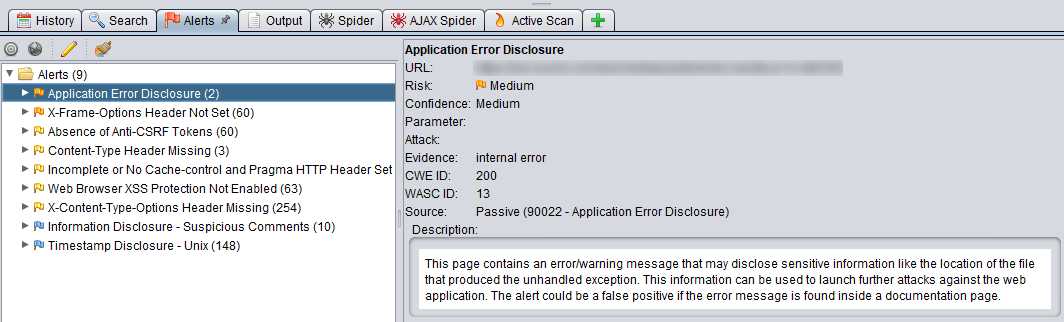
\includegraphics[width=17cm]{zap_example_report.png}
\end{center}
\caption[ZAP report structure example]{ZAP report structure example}
%Source:
\end{figure}

After spidering, scanning and attacking a web application, ZAP provides a report that summarizes different alerts with their severity, the confidence that this problem is present and a possible solution. This information can be used to define whether certain requirements are fulfilled or not.


\subsection{Drawbacks of automated testing}
\label{drawbackAutomated}
At first, automating security tests sounds feasible. Considering the sheer complexity of applications and their possibly infinite attack surface, however, it becomes clear that using automation faces many challenges \citep{stefinko2016}.
A general problem with automated tests is the possibility and, often, a high amount of false positives. 

Especially automated penetration tests lack the experience and intellect of a professional tester that uses pivoting to attack the network and other machines once one machine is compromised \citep{stefinko2016}.
Most popular test automation tools can only leverage vulnerabilities that have already been reported \citep{autoPentestOverview2018}. One of the most significant risks of relying on automated testing is the false sense of security and invincibility that can result from withstanding a defined range of security testing. Real attacks are more complex and can leverage unexpected attack vectors \citep{stefinko2016}.


\section{Related Work}
\label{relatedWork}
The need for novel approaches and automation for security testing becomes present when observing the wide variety of papers published on according ideas and frameworks.
The idea to use similar approaches to security testing based on software functional testing is prominent in model-based testing described in, for example, \citep{torxAMBT2003}. It introduces an abstract framework for automated model-based testing, which can be adapted for security-related topics.
Other approaches, like planning-based testing, as described in \ref{planningBased}, introduce planners and a specific language to describe attack vectors. The implementation of PLAN4SEC in \citep{wotawa2014} provides both examples of a possible framework and the effectiveness of such an approach.

When looking at more concrete implementations for cloud \citep{cloudSec2017} and mobile application \citep{androidTesting2012} security testing, awareness for the enormous value of automating those repetitive processes with a rerunnable continuous deployment emerges. More complex topics, such as automated penetration testing, however, need a lot more research and, most likely, the usage of specialized AI systems in order to provide better and more reliable results than efforts recorded in \citep{autoPentestOverview2018} and \citep{automatedPentesting2011}.


\section{Evaluating and selecting a suitable approach}
The wide range of possible approaches opens up the discussion about which is the \enquote{right one}. Model- and planning-based approaches may provide more reliable results in the long run. However, since the goal of this thesis is to implement and evaluate tooling to test both infrastructures with an underlying defined configuration, and application which comes with the drawbacks explained in \ref{relatedWork}, a more general approach to test automation with \enquote{custom scripts} is taken.

\ref{infrastructure_testing} introduces the underlying concept of infrastructure testing. Compared to security vulnerability testing (\ref{securityVulnerabilityTesting}), a more model-driven approach is already present and provided by cloud providers. The scope of interaction is restricted, which reduces complexity and enables high confidence evaluations to be tested resources.
Considering those advantages, a custom interactor for the Microsoft Azure Policy service was implemented.

Keeping the abstraction on a high level and leveraging the application universality of the ZAP Proxy allows the application level microservice to run a baseline of general tests against any web application. This, however, increases the number of false negatives and reduces the amount of found application-specific vulnerabilities.
For the first proof of concept implementation, this is feasible and can be improved upon functional validation of the setup.

An additional microservice for more specific tests of HTTP responses - like checking for required headers in HTTPS requests - is also added to the system. As described in \ref{customTestingScript}, it holds a mapping between some internal requirements and an execution flow on how to test the given requirement according to application.

All decisions have been taken with consideration on the requirements maintained in SecurityRAT and adjusted towards a consistent architecture and usage described in \ref{extendability}.